\section{Створення панорамного знімку}

Часто бувають ситуації, коли для запису лекції використовується камера з
невисокою роздільною здатністю, через що виникає необхідність рухати
камеру, тому написи, які були на дошці, перестають бути видимими для
глядачів, які не встигли записати матеріал, що було тільки-но
представлено. Рішенням цієї та інших пов'язаних з тремтінням
камери проблем є побудова панорами, яка створюється шляхом склеювання
та накладання кадрів з відео.

\begin{figure}[H]
    \centering
    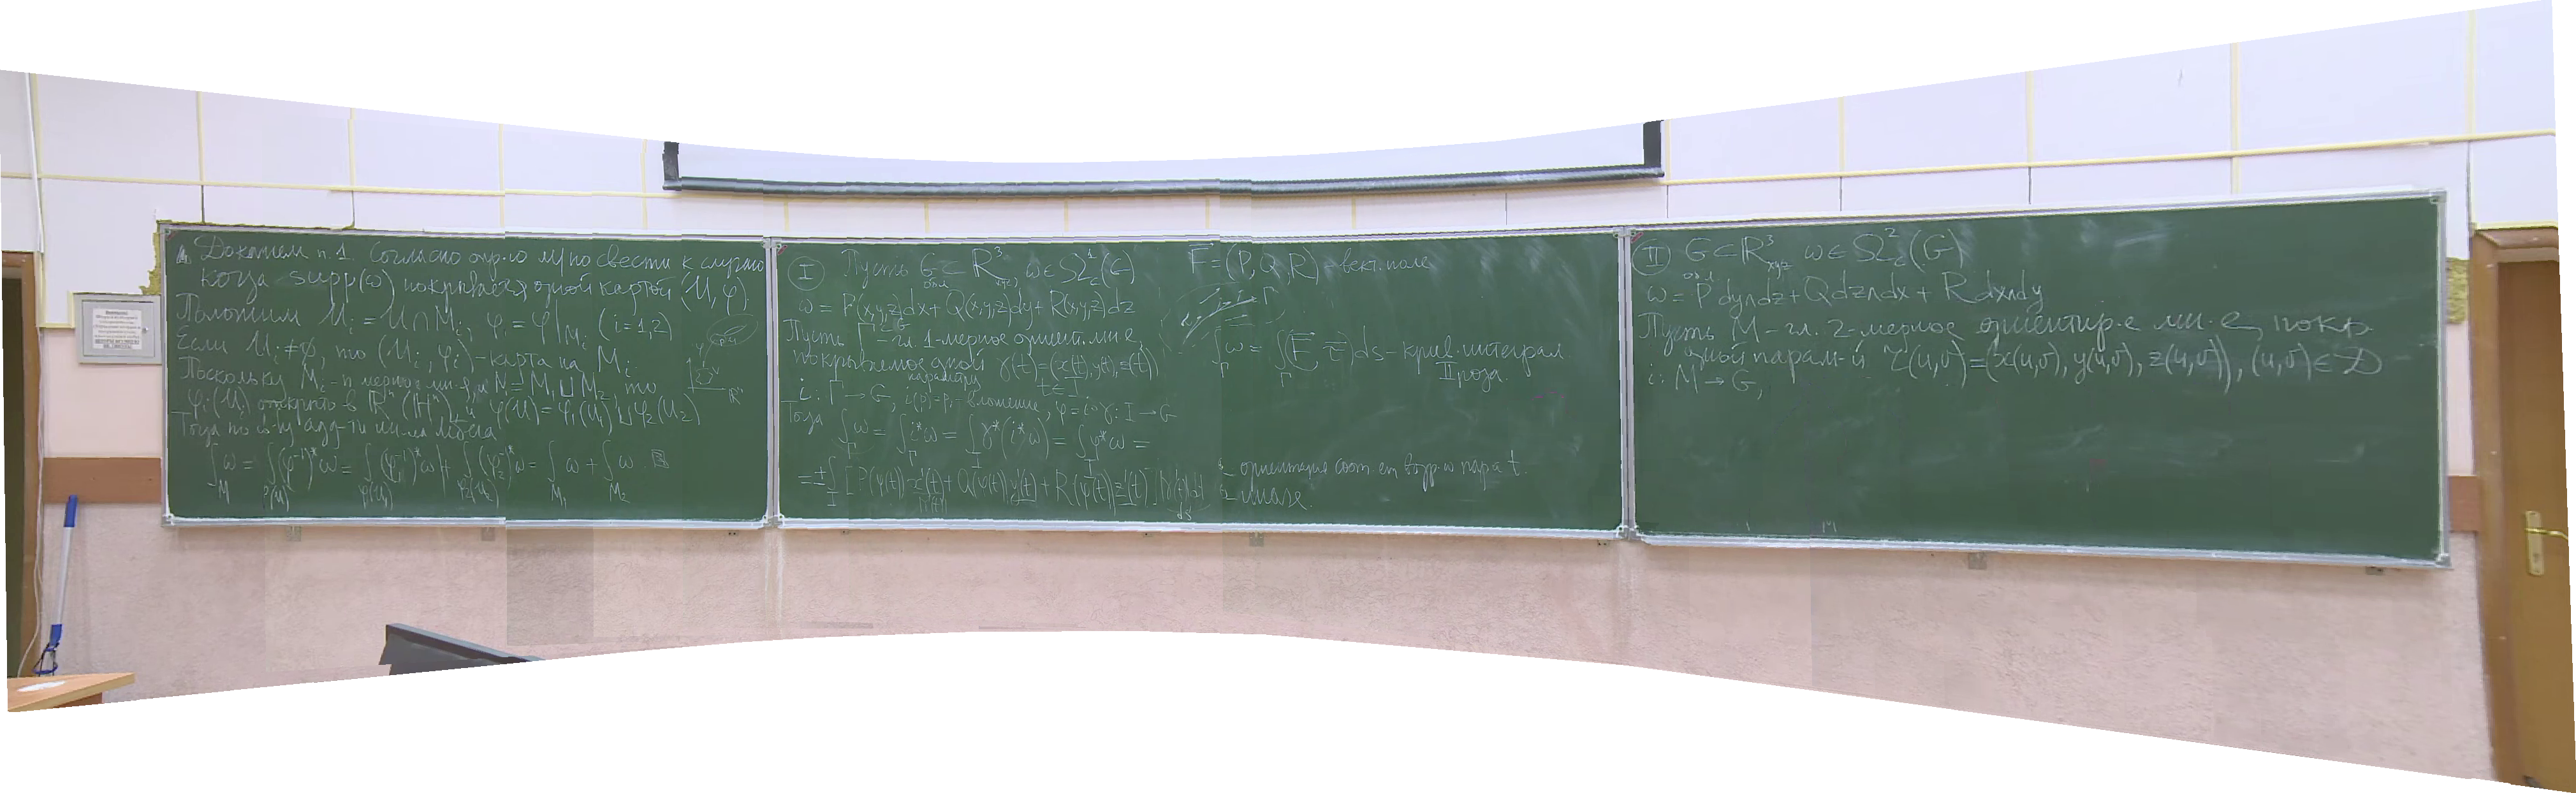
\includegraphics[width=0.8\textwidth]{images/panorama_example}
    \caption{Приклад отриманої панорами з автоматичним видаленням 
    викладача з відео \cite{fpmi_2021_video}
    \label{fig:panorama_example}
    }
\end{figure}

Панорамою \(W^{i}\) називатимемо відображення
\(W^{i}:P_{W}^{i} \rightarrow C\) з множини
\(P_{W}^{i} = \left\{ 1,\ldots,w^{i} \right\} \times \left\{ 1,\ldots,h^{i} \right\}\)
пікселів у множину \(C\mathbb{\subset R}\) інтенсивностей. Зауважимо, що
у кожної панорами може бути своя ширина \(w^{i} \geq w\) і висота
\(h^{i} \geq h\).

% \subsection{Склейка кадрів відео}
% Для того щоб склеїти два кадри дошки застосовується базовий алгоритм 
% поєднання двох знімків з використанням матриці гомографії та відповідних точок.
% Нехай у нас на вхід є два зображення $I_1$ та $I_2$. Маємо матрицю гомографії 
% переводу точок з $I_1$ та $I_2$ $H_{1}^{2}$

\begin{algorithm}[H]
    \caption{Створення панорами}
    \begin{algorithmic}
        \State \textbf{Вхід:} Два кадри \(F^{i}\) та \(F^{i + s}\), поточна панорама \(W^{i}\) (\(W^{1} = F^{1}\))
        \State \textbf{Вихід:} Панорама \(W^{i + s}\).

        \textbf{Етап отримання відповідних точок}

        \textbf{1.} Знаходимо набір \(M^{i}\) пар відповідних пікселів між кадрами
        \(F^{i}\) і \(F^{i + s}\) і будуємо множину
        \(M^{'i} = \left\{ \left( p^{i},p^{i + s} \right) \in M^{i}:B_{p^{i}}^{i} = B_{p^{i + s}}^{i} = 0 \right\}\)
        тих пар відповідних пікселів, координати яких не належать області
        рухомих об'єктів.

        \textbf{2.}
        Якщо \(\left| {M'}^{i} \right| < 0.5 \cdot \left| M^{i} \right|\) або
        \(\left| {M'}^{i} \right| < 4\), завершуємо алгоритм з результатом
        \(W^{i + s} = W^{i}\).

        \textbf{3.}
        Знаходимо набір \(M_{W}^{i}\) пар відповідних пікселів між панорамою
        \(W^{i}\) і кадром \(F^{i + s}\) і будуємо множину
        \(M_{W}^{'i} = \left\{ \left( p_{W}^{i},p^{i + s} \right) \in M_{W}^{i}:\exists p^{i} \in P:\left( p^{i},p^{i + s} \right) \in M^{'i} \right\}\).
        
        \textbf{Етап обчислення матриці гомографії}

        \textbf{4.}
        На базі множини \(M_{W}^{'i}\) пар відповідних точок знаходимо матрицю
        \(H_{W}^{i}\) гомографії, що співставляє пікселі кадру \(F^{i + s}\)
        та панорами \(W^{i}\).

        \textbf{Етап обчислення розміру нової панорами}

        \textbf{5.}
        Рахуємо координати
        \(l_{1}^{i} = H_{W}^{i} \cdot (0,0,1)^{T}\),
        \(l_{2}^{i} = H_{W}^{i} \cdot (w - 1,0,1)^{T}\),
        \(l_{3}^{i} = H_{W}^{i} \cdot (0,h - 1,1)^{T}\),
        \(l_{4}^{i} = H_{W}^{i} \cdot (h - 1,h - 1,1)^{T}\) крайніх
        точок кадру \(F^{i + s}\) після застосування до них матриці
        \(H_{W}^{i}\).

        \textbf{6.}
        Для визначення множини \(P_{W}^{i}\) нової панорами \(W^{i + s}\)
        рахуємо величини
        \(x_{\min}^{i} = \min_{j = \overline{1,4}}\frac{( l_{j}^{i} )_{x}}{( l_{j}^{i} )_{z}}\),
        \(x_{\max}^{i} = \max_{j = \overline{1,4}}\frac{( l_{j}^{i} )_{x}}{( l_{j}^{i} )_{z}}\),
        \(y_{\min}^{i} = \min_{j = \overline{1,4}}\frac{( l_{j}^{i} )_{y}}{( l_{j}^{i} )_{z}}\),
        \(y_{\max}^{i} = \max_{j = \overline{1,4}}\frac{( l_{j}^{i} )_{y}}{( l_{j}^{i} )_{z}}\).
        Позначимо
        $P_{W}^{i + s} = 
        { 1,\ldots,\max( w^{i},x_{\max}^{i} - x_{\min}^{i} ) }
        \times 
        { 1,\ldots,\max( h^{i},y_{\max}^{i} - y_{\min}^{i} ) }$.

        \textbf{Етап створення нової панорами}
        
        \textbf{7.}
        Будуємо панораму $W^{i+s}$. Для зручності позначимо обернену матрицю $H^{'} = (H_{W}^{i})^{-1}$, числа
        $x_{\min}^{'} = \min(x_{\max}^{i}, 0), y_{\min}^{'} = \min(y_{\max}^{i}, 0)$ і відображення
        $f^i: p \rightarrow
            (|\frac{(H^{'} \cdot p)_x}{(H^{'} \cdot p)_y}|, |\frac{(H^{'} \cdot p)_y}{(H^{'} \cdot p)_z}|)$, що перетворює
        координати з панорами до пікселів кадру за допомогою гомографії. Інтенсивність у пікселі $p$ панорами
        $W^{i+s}$ визначається за формулою

        \begin{equation*}
            W^{i + s}(p) =
            \begin{gathered}
                \begin{cases}
                    F^{i + s}(f(p)),                            & f(p) \in P,                                    \\
                    W^{i}( p + ( x_{\min}^{'},y_{\min}^{'} ) ), & p + ( x_{\min}^{'},y_{\min}^{'} ) \in P^{i},   \\
                    0,                                          & p + ( x_{\min}^{'},y_{\min}^{'} ) \notin P^{i}
                \end{cases}
            \end{gathered}
        \end{equation*}
    \end{algorithmic}
    \label{al:panorama_creating_algorithm}
\end{algorithm}

\clearpage
